\documentclass{beamer}

\mode<presentation>
{
  \usetheme{Frankfurt}
  \usecolortheme{beaver}
  \setbeamercovered{transparent}
  \useoutertheme{split}
  \setbeamertemplate{footline}[page number]{}
  \setbeamertemplate{navigation symbols}{} 
}

\usepackage{multirow}

\usepackage[english]{babel}
\usepackage[utf8]{inputenc}
\usepackage{times}
\usepackage[T1]{fontenc}

\usepackage{color, colortbl}

\definecolor{LightGray}{gray}{.9} % for table rows

\usepackage{graphics}

\usepackage[absolute,overlay]{textpos}
\newenvironment{reference}[2]{%
  \begin{textblock*}{\textwidth}(#1,#2)

      \tiny\it\bgroup\color{red!50!black}}{\egroup\end{textblock*}}

\title{Mesh Adaptation Based on the Depth Image (MABDI)}

\author{
{Lucas Chavez} \\ ~\\
{\small{Dr. Lumia\inst{1} \and Dr. Fierro\inst{1} \\ \and Dr. Chaimowicz\inst{2} \and
Dr. Campos\inst{2} \and Dr. Anderson\inst{3}}} 
}

\titlegraphic{
   
\includegraphics[height=1cm]{logo.jpg} \hspace{.3in}
   
\includegraphics[height=1cm]{verlab.pdf} \hspace{.3in}
   
\includegraphics[height=1cm]{sandia.pdf}
}

\institute
{
  \inst{1}%
  University of New Mexico  \and
  \inst{2}%
  Universidade Federal de Minas Gerais \and
  \inst{3}%
  Sandia National Laboratories 
}

\date{April 2013}

% \pgfdeclareimage[height=0.5cm]{university-logo}{university-logo-filename}
% \logo{\pgfuseimage{university-logo}}

% Delete this, if you do not want the table of contents to pop up at
% the beginning of each subsection:
\AtBeginSection[]
{
  \begin{frame}<beamer>{Outline}
    \tableofcontents[currentsection,currentsubsection]
  \end{frame}
}


% If you wish to uncover everything in a step-wise fashion, uncomment
% the following command: 
%\beamerdefaultoverlayspecification{<+->}

\begin{document}

\begin{frame}[plain]
  \titlepage
\end{frame}

\begin{frame}{Outline}
  \tableofcontents
  % You might wish to add the option [pausesections]
\end{frame}

\section{Introduction}

\subsection{Goal}

\begin{frame}{What is the main objective?}
\begin{reference}{4mm}{90mm}
(Marton et al. 2009) On Fast Surface Reconstruction Methods for Large and Noisy Point Clouds
\end{reference} 
  {\small RGB-D sensor to make a useful representation of the environment}
  \vspace{-.2in}
  \begin{center}
  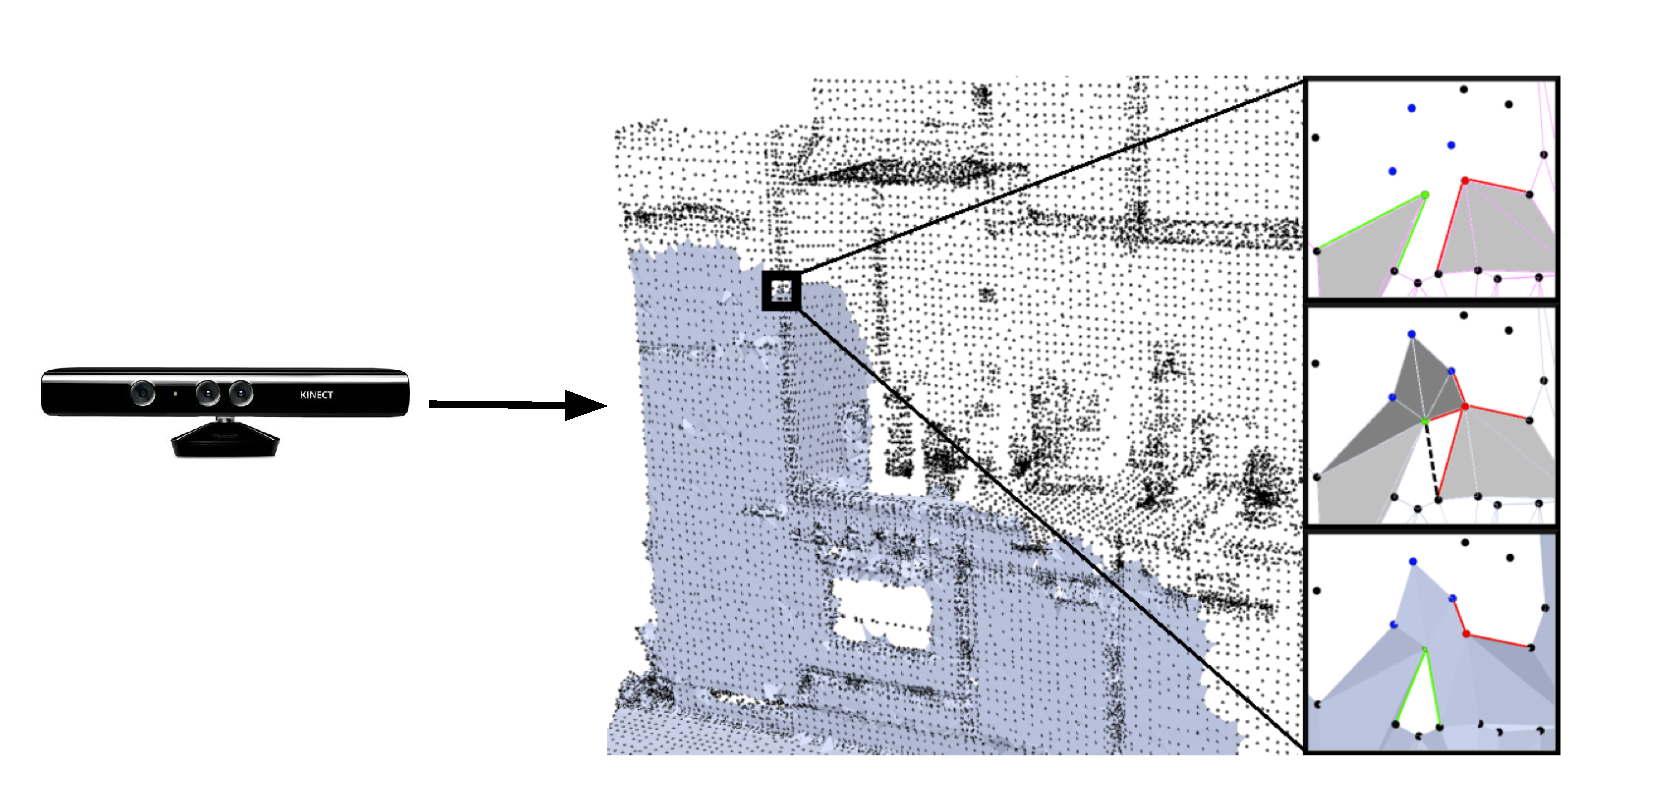
\includegraphics[height=5.9cm]{MainGoal.pdf} 
  \end{center}
\end{frame}

\subsection{Motivation}

\begin{frame}{What can representation like this be used for?}
\begin{reference}{4mm}{88mm}
(Berenson et. al 2012) A robot path planning framework that learns from experience \\
(Kadous et. al 2006) Effective user interface design for rescue robotics
\end{reference} 
\begin{columns}
\column{.50\textwidth}
Robotic applications
  \begin{center}
  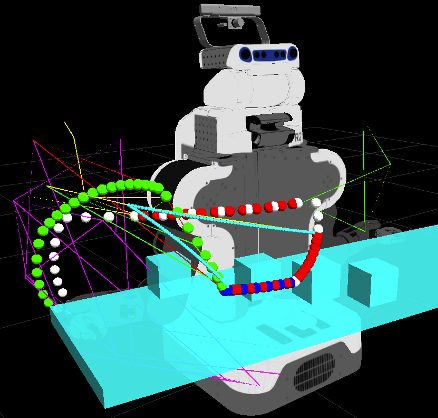
\includegraphics[width=\textwidth]{m_r.png} 
  \end{center}
\column{.50\textwidth}
Urban search and rescue (USAR)
  \begin{center}
  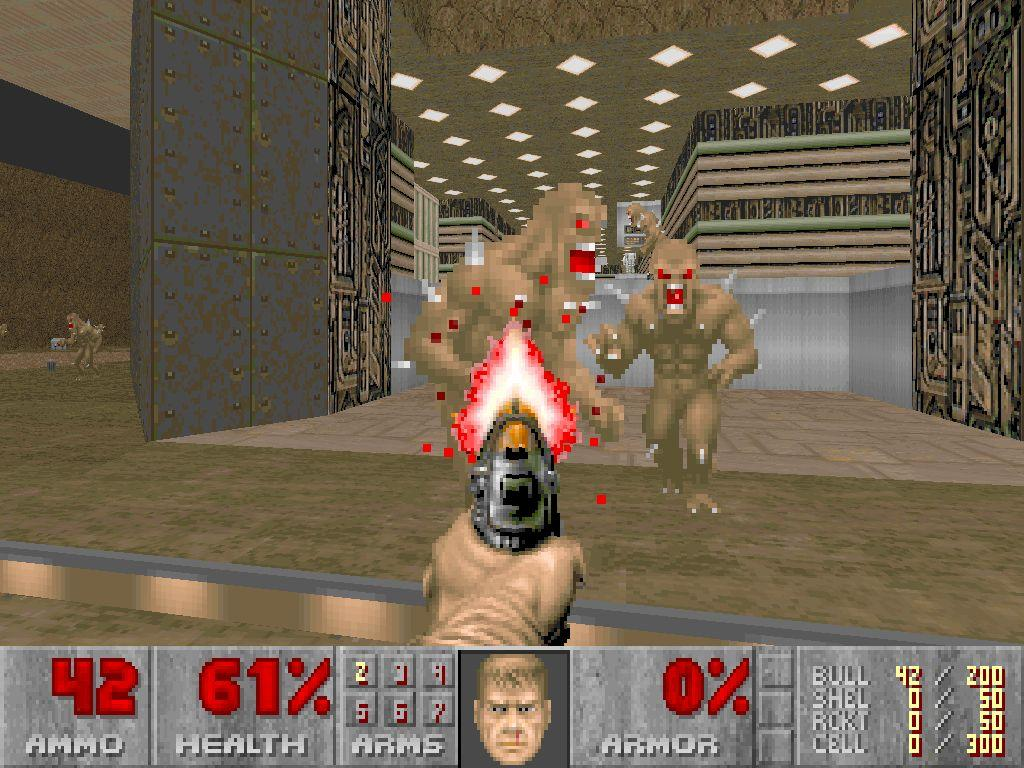
\includegraphics[width=\textwidth]{m_usar.jpg} 
  \end{center}
\end{columns}
\end{frame}

\subsection{History}

\begin{frame}{Comparing the different representations}
{
\oddsidemargin -0.9in
\color{black}
\begin{table}[h]
\begin{footnotesize}
\begin{center}
\begin{tabular}{|l|c|c|c|c|c|}
\hline
\multirow{2}{*}{} & Adaptability & Computationally & Low Memory & SA: & SA: \\
 & & Inexpensive & Requirement & Robot & Human \\\hline
Landmark Locations  	& x & x & x & - & - \\
Point Clouds		& - & x & - & - & - \\
Surfels             	& x & x & x & - & x \\
Implicit Functions 	& x & - & - & x & x \\
Static Mesh	 	& - & x & x & x & x \\
Adaptive Mesh	 	& x & o & o & x & x \\
\hline
\end{tabular}
\end{center}
\end{footnotesize}
\end{table}
}
\vspace{-.5in}
Desired representation methodology characteristics:
\begin{itemize}
\item Adapt existing mesh with new measurements
\item Quickly identify new parts of the scene
\item React to new or removed objects
\item Computationally and memory efficient
\end{itemize}
\end{frame}

\begin{frame}{Related works}
Surface Reconstruction - Computer Graphics \& Computational Geometry (Seitz
2006; Mencl 1997) 
\begin{itemize}
\item Volume-based
\item Signed Distance Function (Ohtake 2003)
\item Surface-based
\item Incremental Surface Growing (Marton 2009)
\end{itemize}
~\\
Simultaneous Localization and Mapping (SLAM)
\begin{itemize}
\item Probabilistic Geometry Estimation (Cashier 2012)
\item Kintinuous (Whelan et. al 2012)
\item KinectFusion (Newcombe et. al 2011)
\item RGB-D Mapping (Henry et al. 2010)
\end{itemize}
\end{frame}


\section{Approach}

\subsection{Idea}

\begin{frame}{What do I intend to do different?}
The main idea is to leverage fast image processing techniques
\begin{itemize}
\item Works well with GPU
\item Depth image contains lots of information
\vspace{.1in} 
\end{itemize}
Want to categorize measurements and define connectivity 
\begin{itemize}
\item Connectivity defined in depth image is preserved 
\item Measurements need to be categorized
\begin{itemize}
\item $D_u$ - unseen
\item $D_s$ - supporting 
\begin{itemize}
\item $D_n$ - new object
\item $D_r$ - removed object
\end{itemize}
\end{itemize}
\end{itemize}
\end{frame}

\subsection{System}

\begin{frame}{How will it work?}
\vspace{-.2in}
  \begin{center}
\begin{table}[h]
\begin{footnotesize}
\begin{center}
\begin{tabular}{|c|l|}
\hline
{\bf Variable Name} & \multicolumn{1}{|c|}{{\bf Description}} \\
\hline
\rowcolor{LightGray} $D$ & Depth image from RGB-D sensor \\ 
$F$ & Frequency response image \\
\rowcolor{LightGray} $K_S,K_L,\text{ and }K_G$ & Image convolution operators \\
$V \text{ and } C$ & Mesh vertices and connectivity of the current triangulation \\
\rowcolor{LightGray} $T$ & Current triangulation. Contains both $V$ and $C$ \\
$P$ & The known pose of the sensor \\
\rowcolor{LightGray} $E$ & Expected depth image \\ 
$D_u$ & Previously \emph{unseen} parts of $D$ \\ 
\rowcolor{LightGray} $D_s$ & Parts of $D$ which \emph{support} an existing part of
$M$ \\ 
$D_n$ & Parts of $D$ which correspond to a \emph{new} object \\ 
\rowcolor{LightGray} $D_r$ & Parts of $D$ which correspond to a
\emph{removed} object \\ 
$M$ & Current mesh \\
\hline
\end{tabular}
\end{center}
\label{tab:var}
\end{footnotesize}
\end{table}
  \end{center}
\end{frame}

\begin{frame}{How will it work?}
\vspace{-.2in}
  \begin{center}
  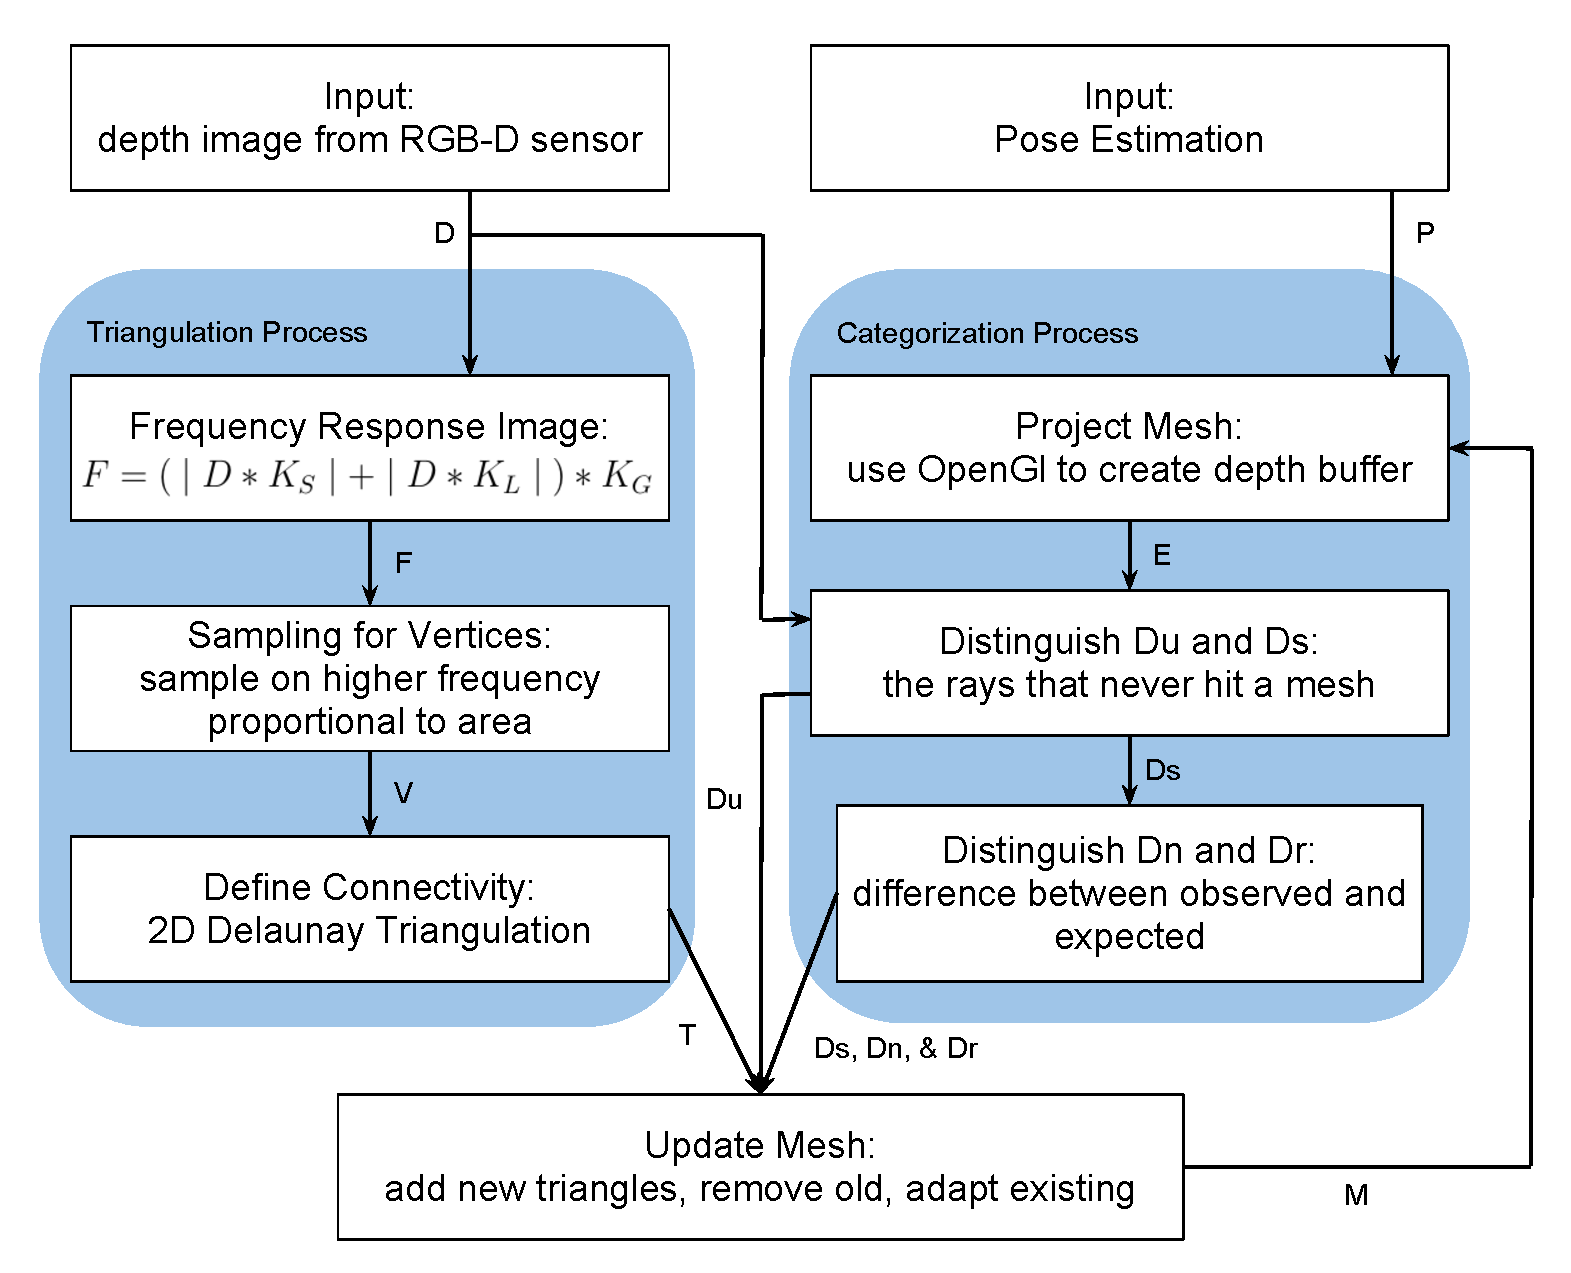
\includegraphics[width=.9\textwidth]{SD.pdf} 
  \end{center}
\end{frame}

\begin{frame}{Input from the RGB-D Sensor}
\vspace{-.1in}
\begin{columns}
\column{.25\textwidth}
  \begin{center}
  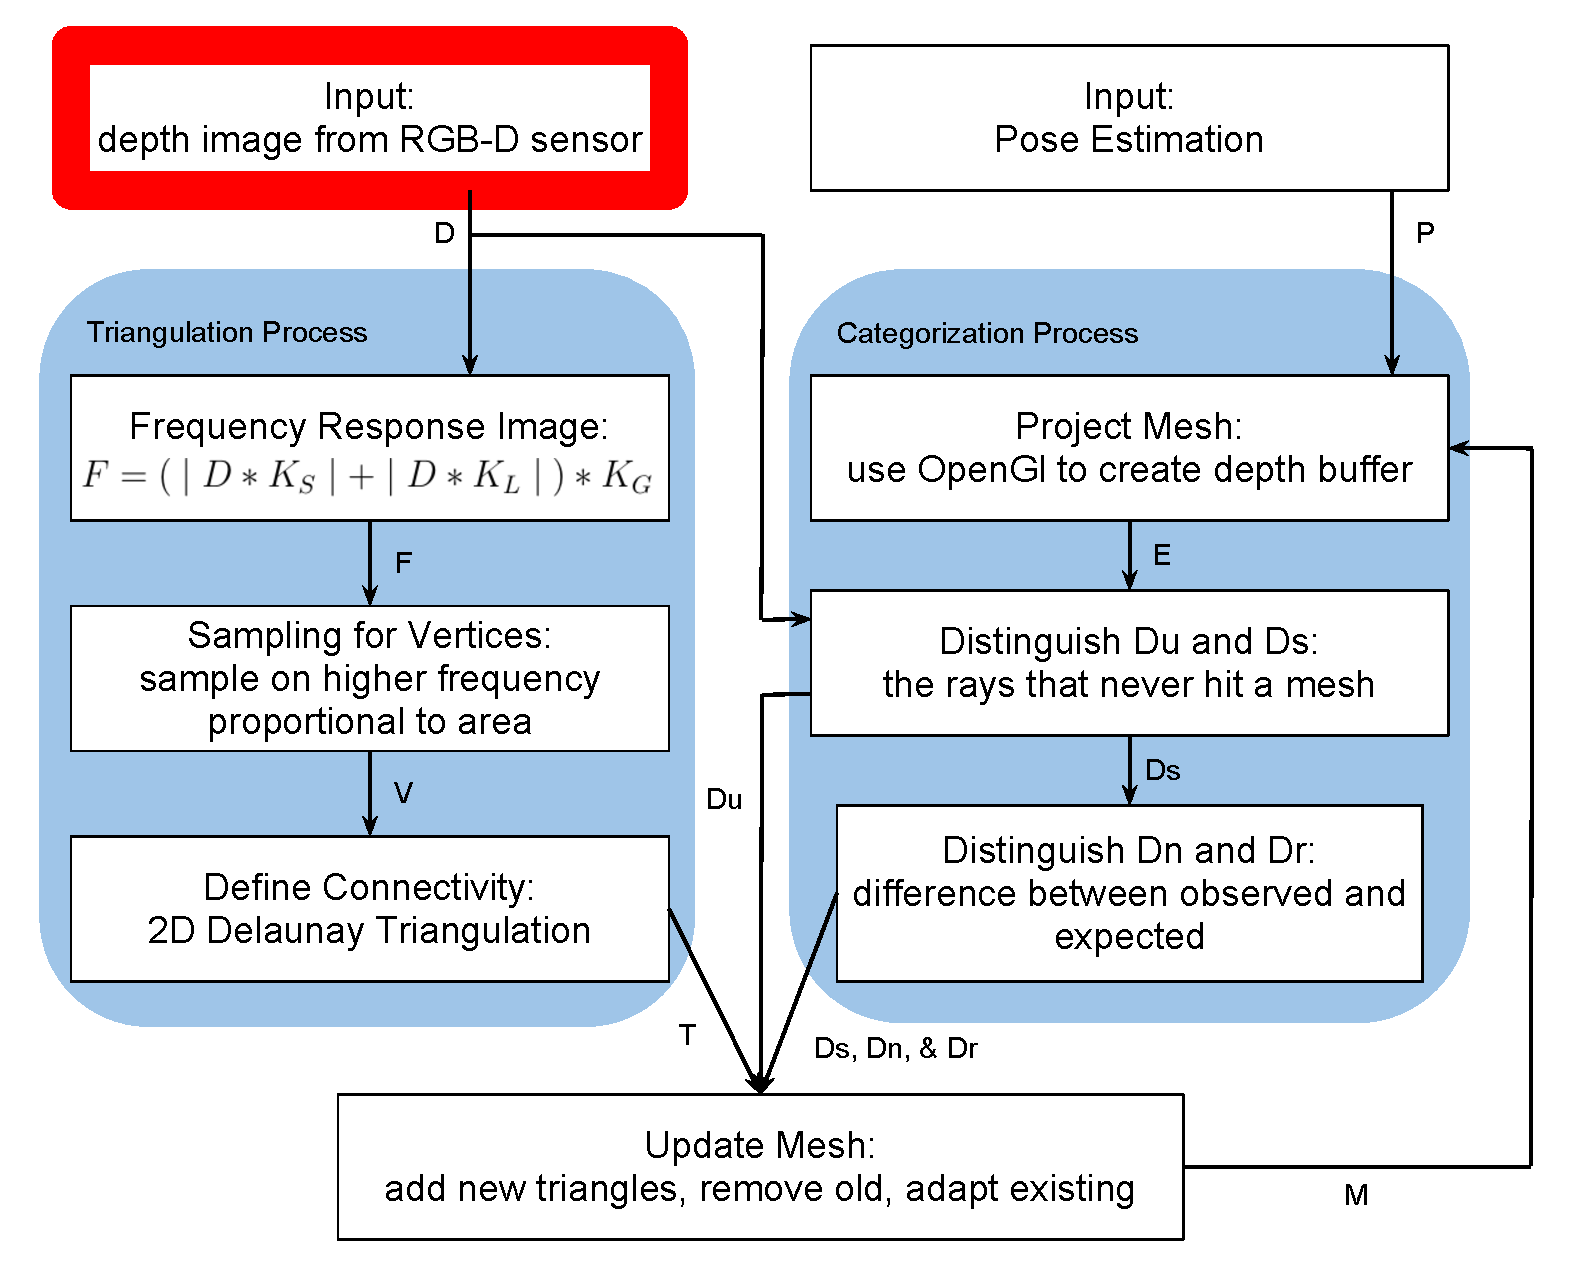
\includegraphics[width=\textwidth]{SDinput.pdf} 
  \end{center}
  \begin{center}
  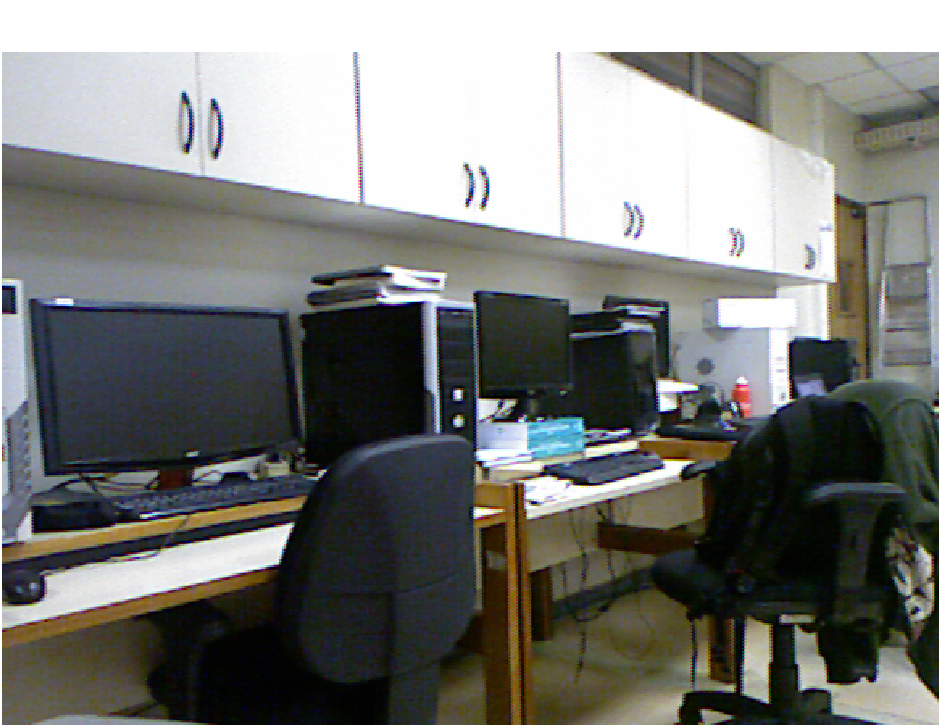
\includegraphics[width=\textwidth]{m_photo.pdf} 
  \end{center}
\column{.75\textwidth}
  \begin{center}
  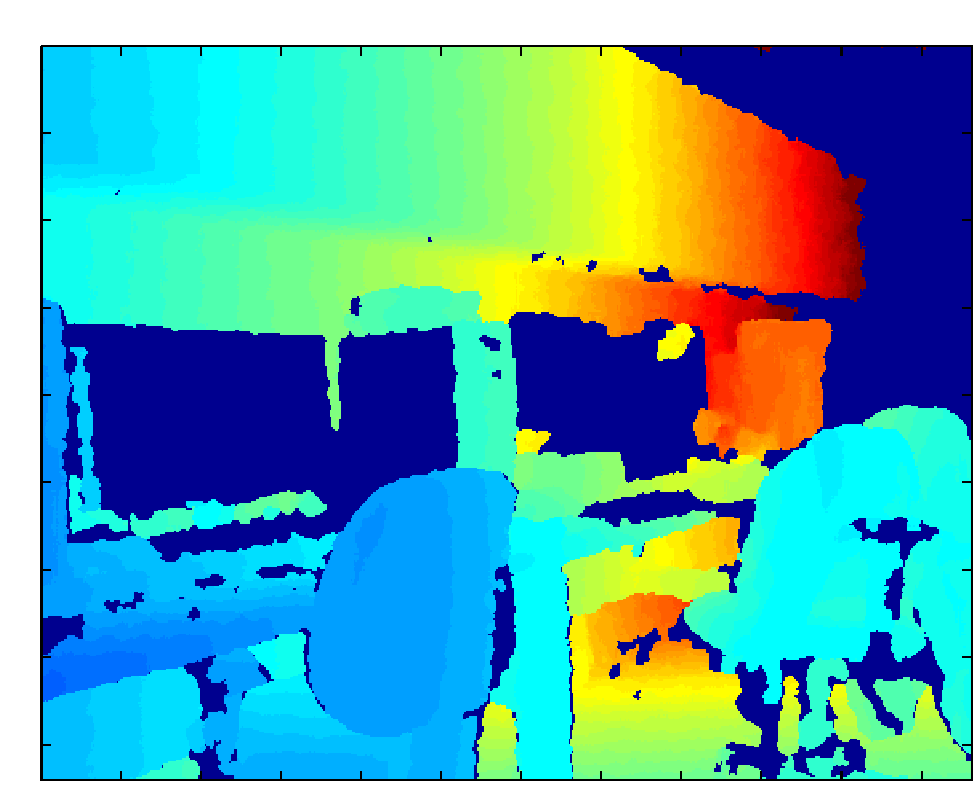
\includegraphics[width=\textwidth]{m_depth.pdf} 
  \end{center}
\end{columns}
\end{frame}

\begin{frame}{I want to know the areas that need more vertices}
\vspace{-.1in}
\begin{columns}
\column{.25\textwidth}
  \begin{center}
  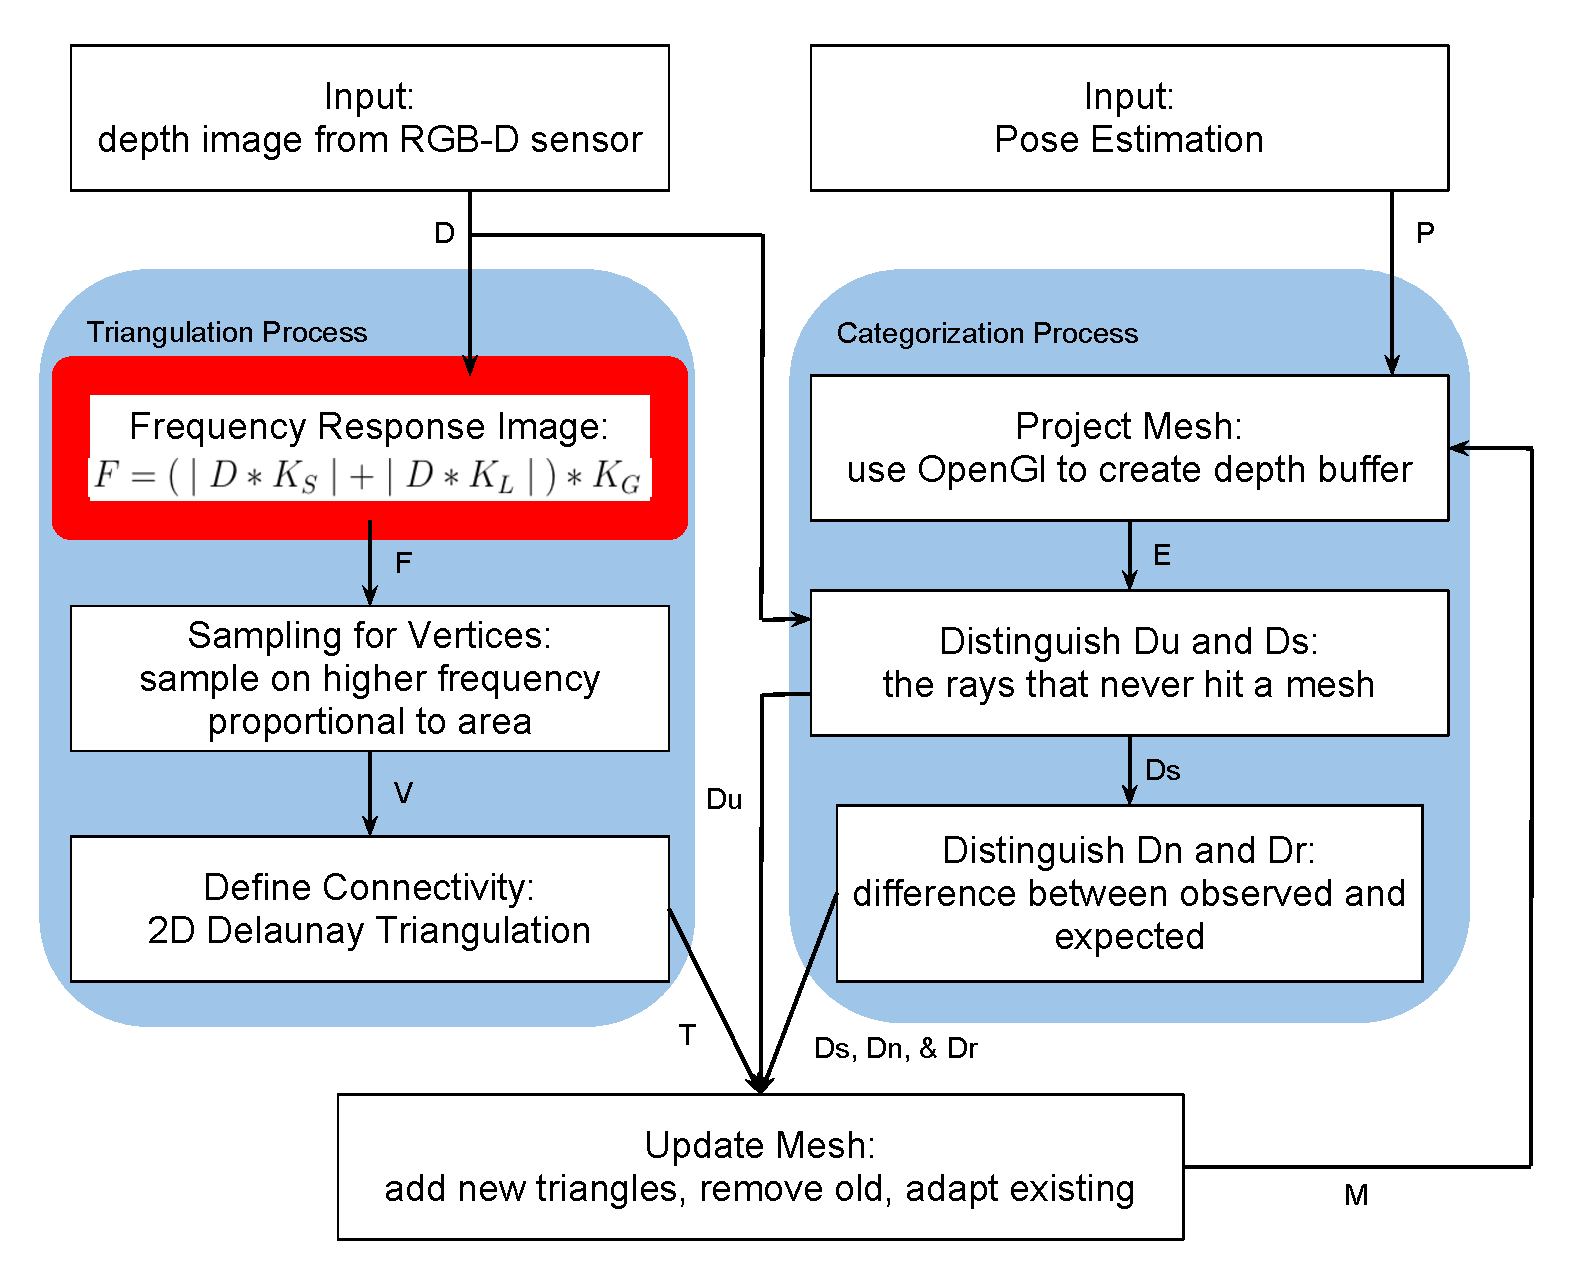
\includegraphics[width=\textwidth]{SDfreq.pdf} 
  \end{center}
\column{.75\textwidth}
  \begin{center}
  $F=(\ \mid D \ast K_S \mid + \mid D \ast K_L \mid \ ) \ast K_G$
  \vspace{-.1in}
  \begin{figure}
  \includegraphics<1>[width=\textwidth]{m_freq.pdf} 
  \includegraphics<2>[width=\textwidth]{m_freqn.pdf} 
  \end{figure}
  \end{center}
\end{columns}
\end{frame}

\begin{frame}{Determine the actual vertices by probabilistic sampling}
\vspace{-.1in}
\begin{columns}
\column{.25\textwidth}
  \begin{center}
  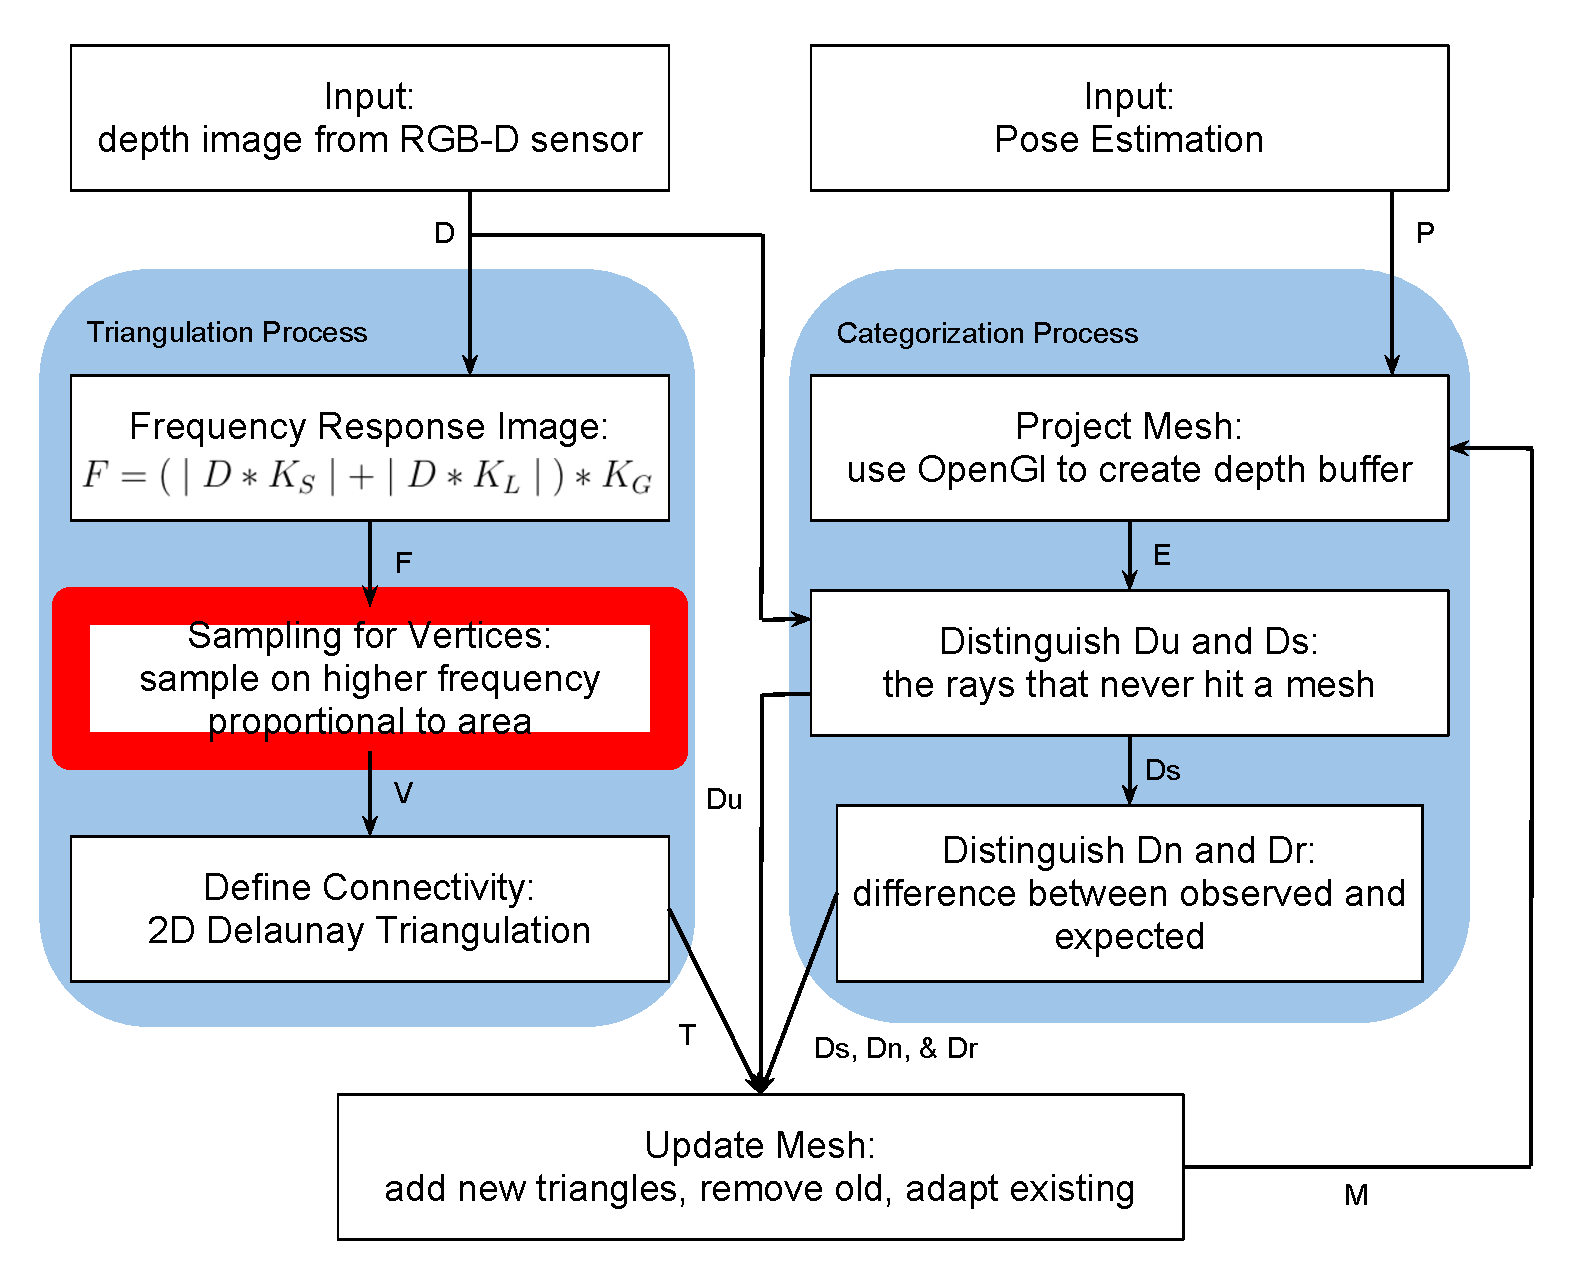
\includegraphics[width=\textwidth]{SDsampling.pdf} 
  \end{center}
\column{.75\textwidth}
  \begin{center}
  \begin{figure}
  \includegraphics<1>[width=\textwidth]{m_fhist.pdf} 
  \includegraphics<2>[width=\textwidth]{m_ihist.pdf} 
  \includegraphics<3>[width=\textwidth]{m_csamples.pdf} 
  \end{figure}
  \end{center}
\end{columns}
\end{frame}

\begin{frame}{Connectivity of triangles $(T)$ with 2D Delaunay}
\vspace{-.1in}
\begin{columns}
\column{.25\textwidth}
  \begin{center}
  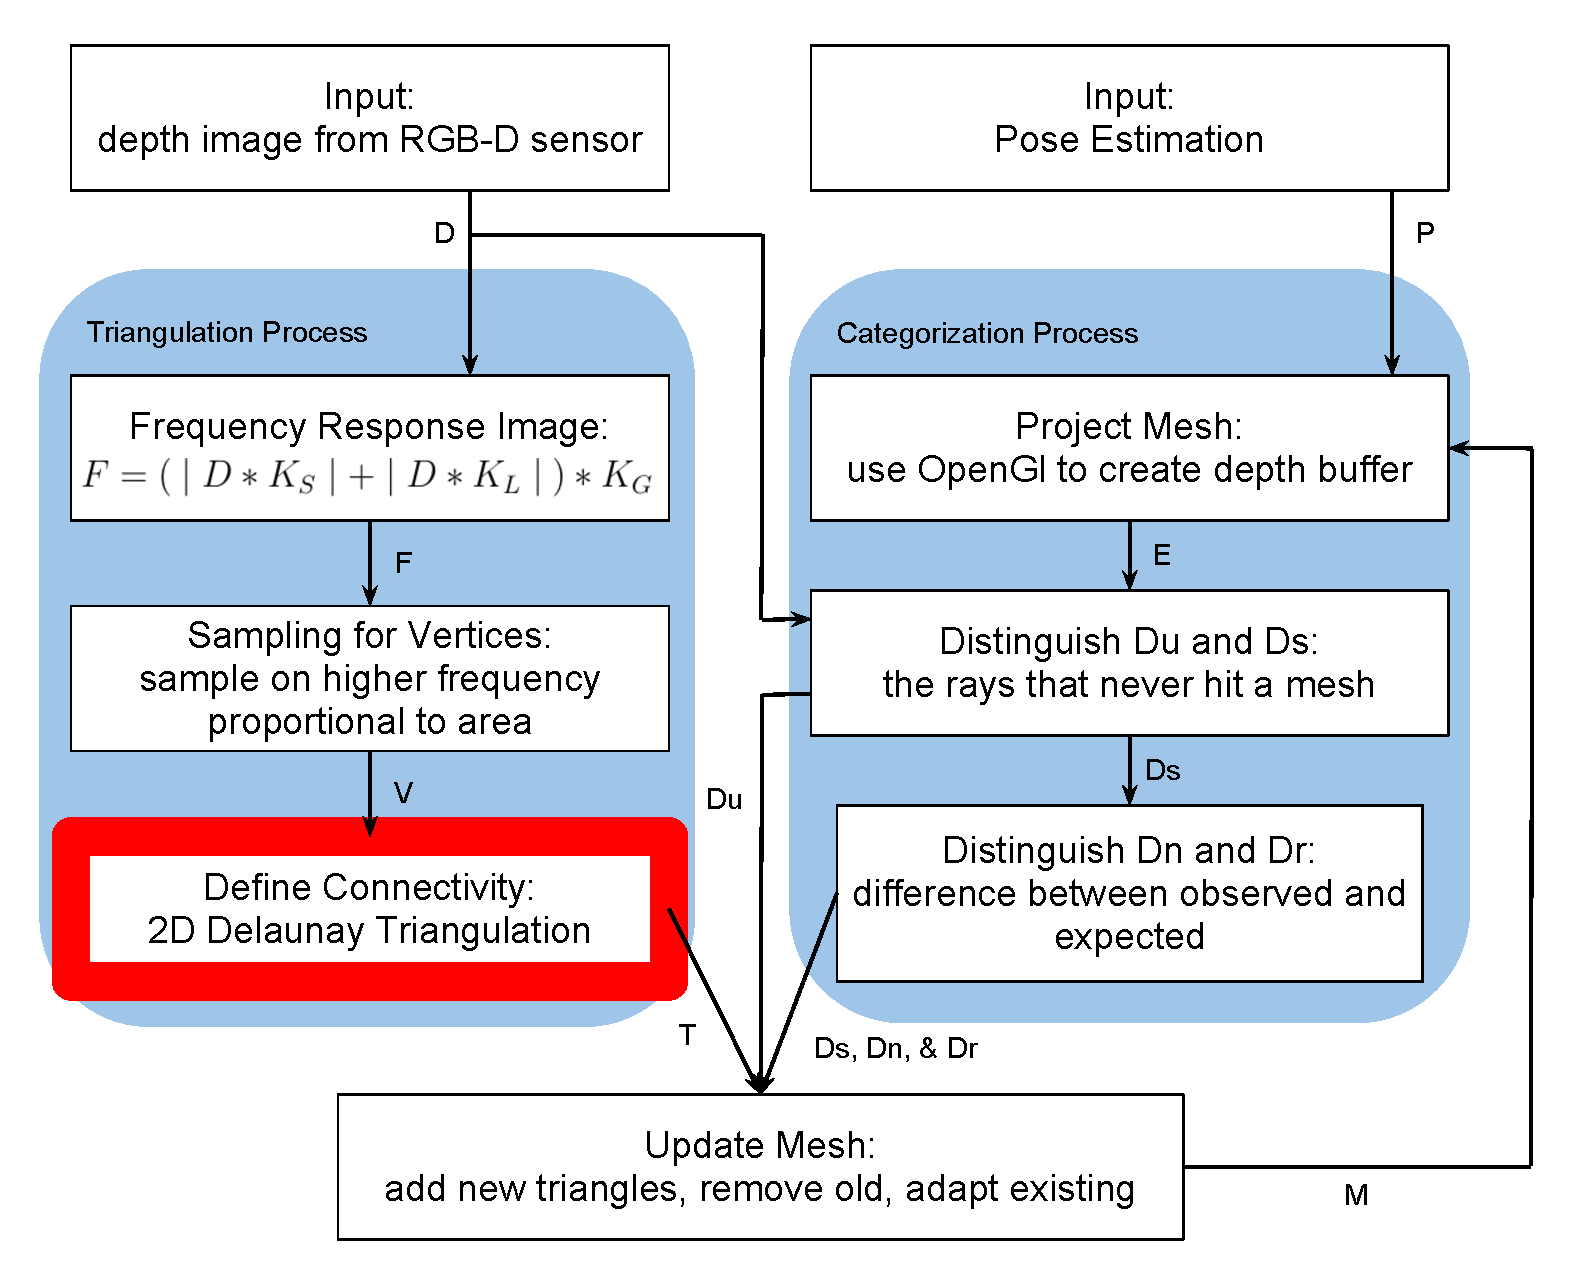
\includegraphics[width=\textwidth]{SDconnect.pdf} 
  \end{center}
\column{.75\textwidth}
  \begin{center}
  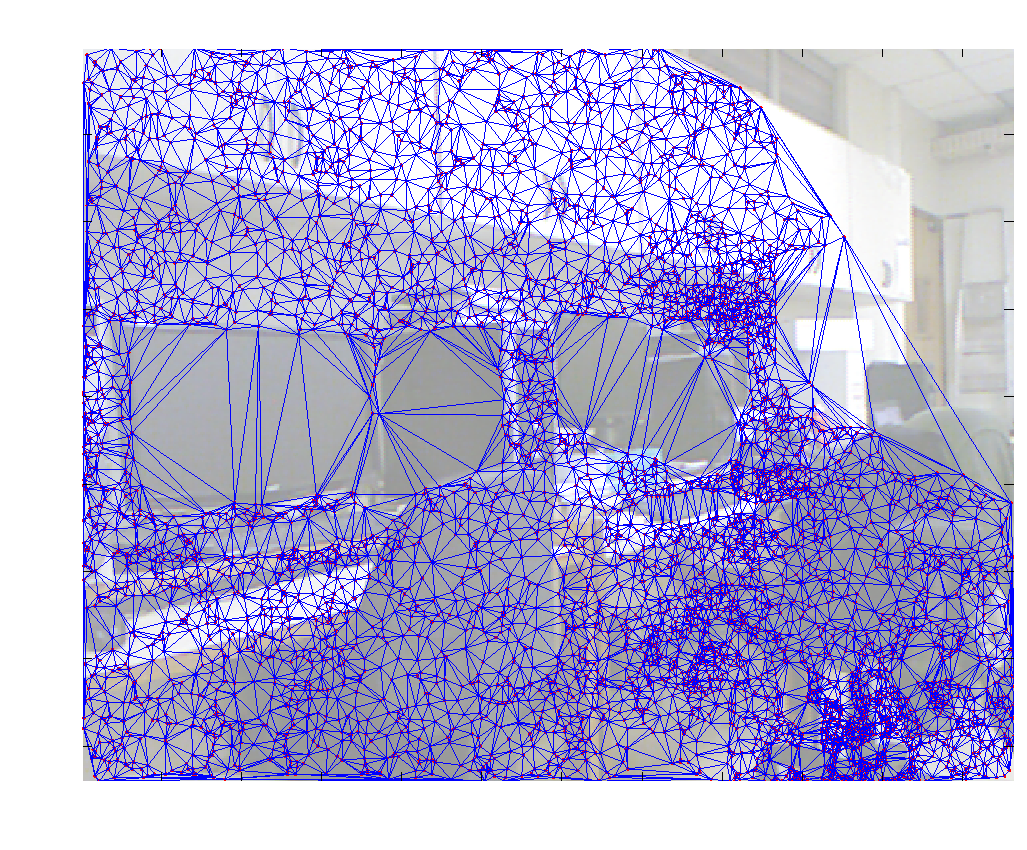
\includegraphics[width=\textwidth]{m_ctr.pdf} 
  \end{center}
\end{columns}
\end{frame}

\begin{frame}{Project existing mesh onto depth image plane}
\begin{reference}{4mm}{92mm}
(Fallon et al. 2012) Efficient scene simulation for robust monte carlo localization using an RGB-D camera
\end{reference} 
\vspace{-.1in}
\begin{columns}
\column{.25\textwidth}
  \begin{center}
  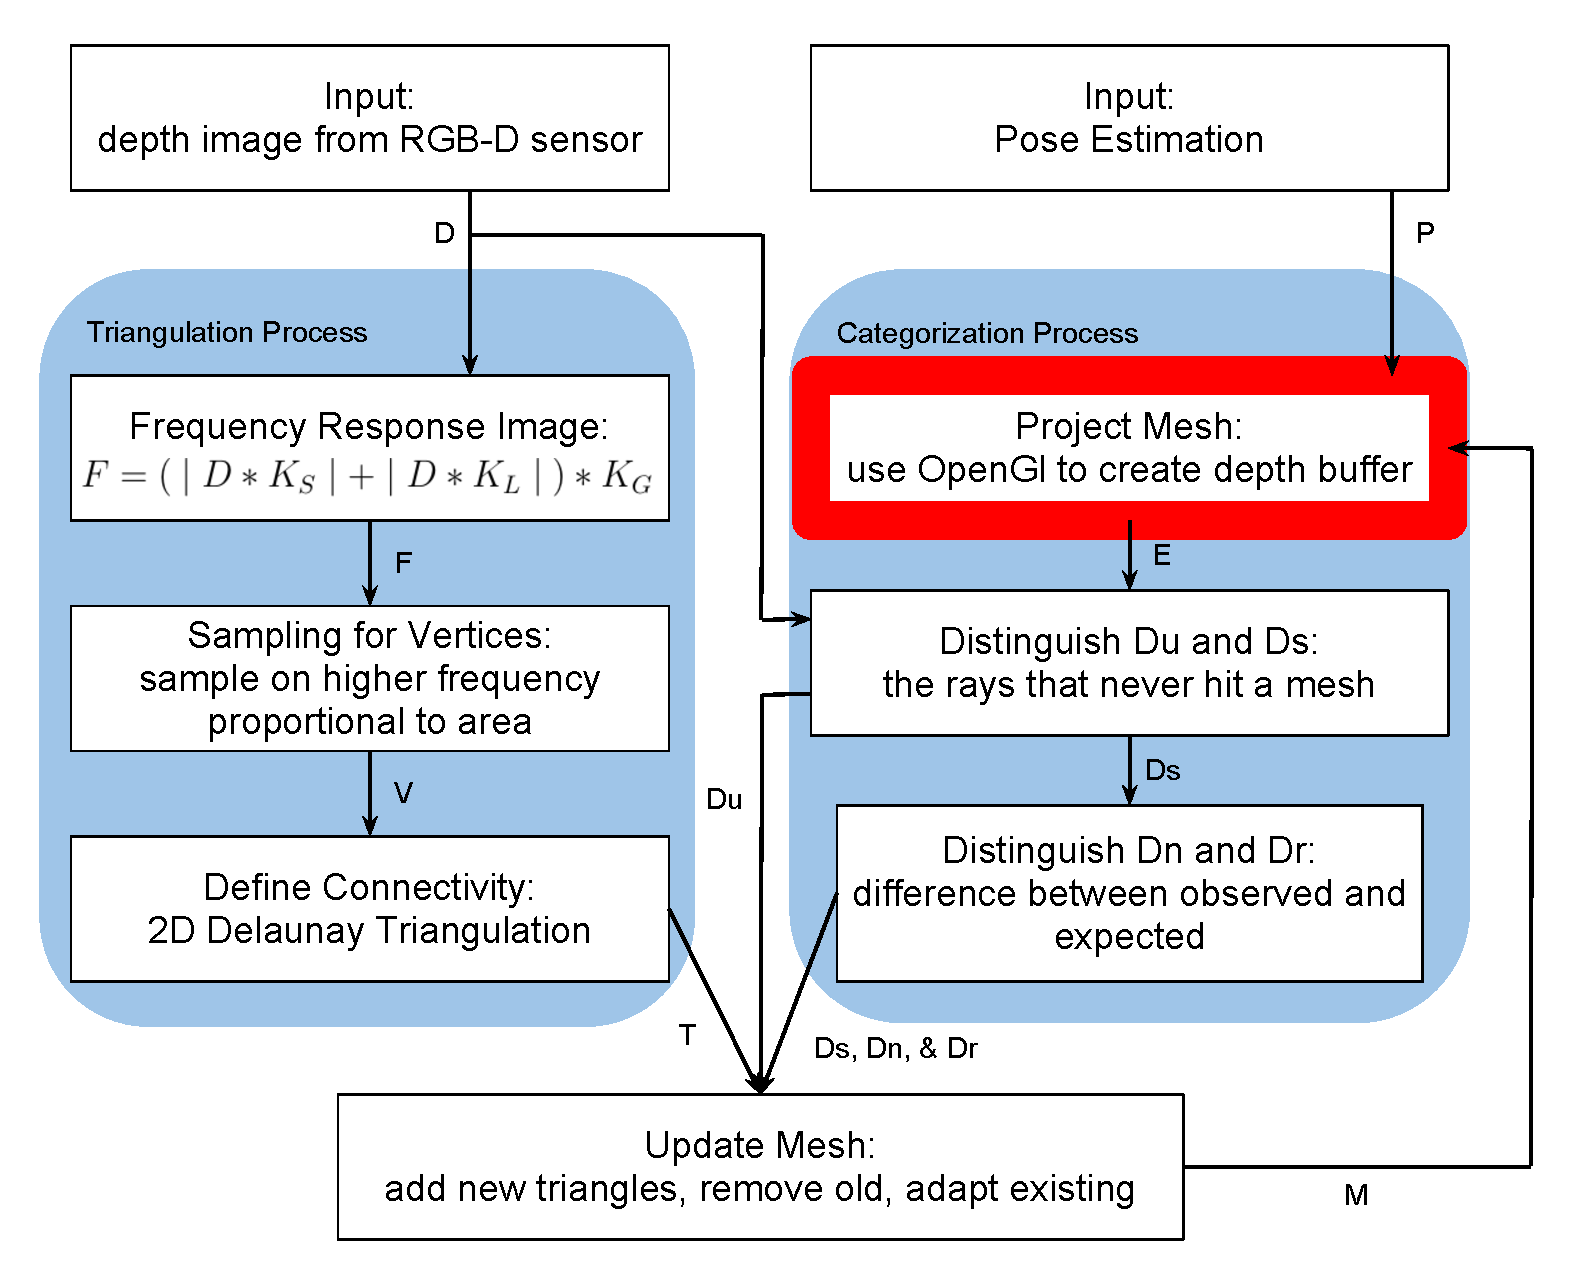
\includegraphics[width=\textwidth]{SDproject.pdf} 
  \end{center}
\column{.75\textwidth}
  This step gives the expected measurements $E$
  \vspace{-.1in}
  \begin{center}
  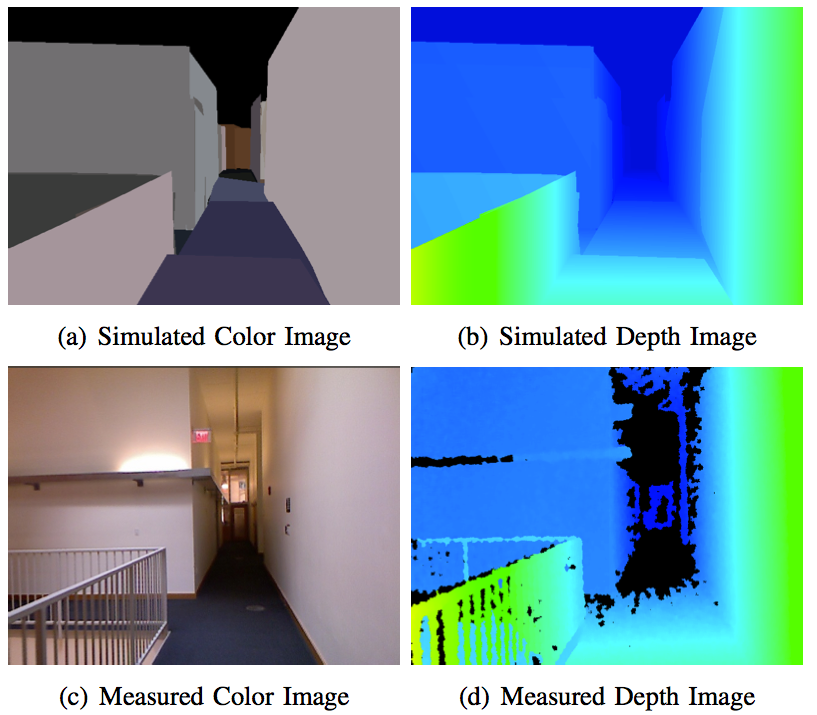
\includegraphics[width=.9\textwidth]{m_proj.png} 
  \end{center}
\end{columns}
\end{frame}

\begin{frame}{Categorize measurements into $D_u,\ D_s,\ D_n,\ \& \ D_r$}
\vspace{-.1in}
\begin{columns}
\column{.25\textwidth}
  \begin{center}
  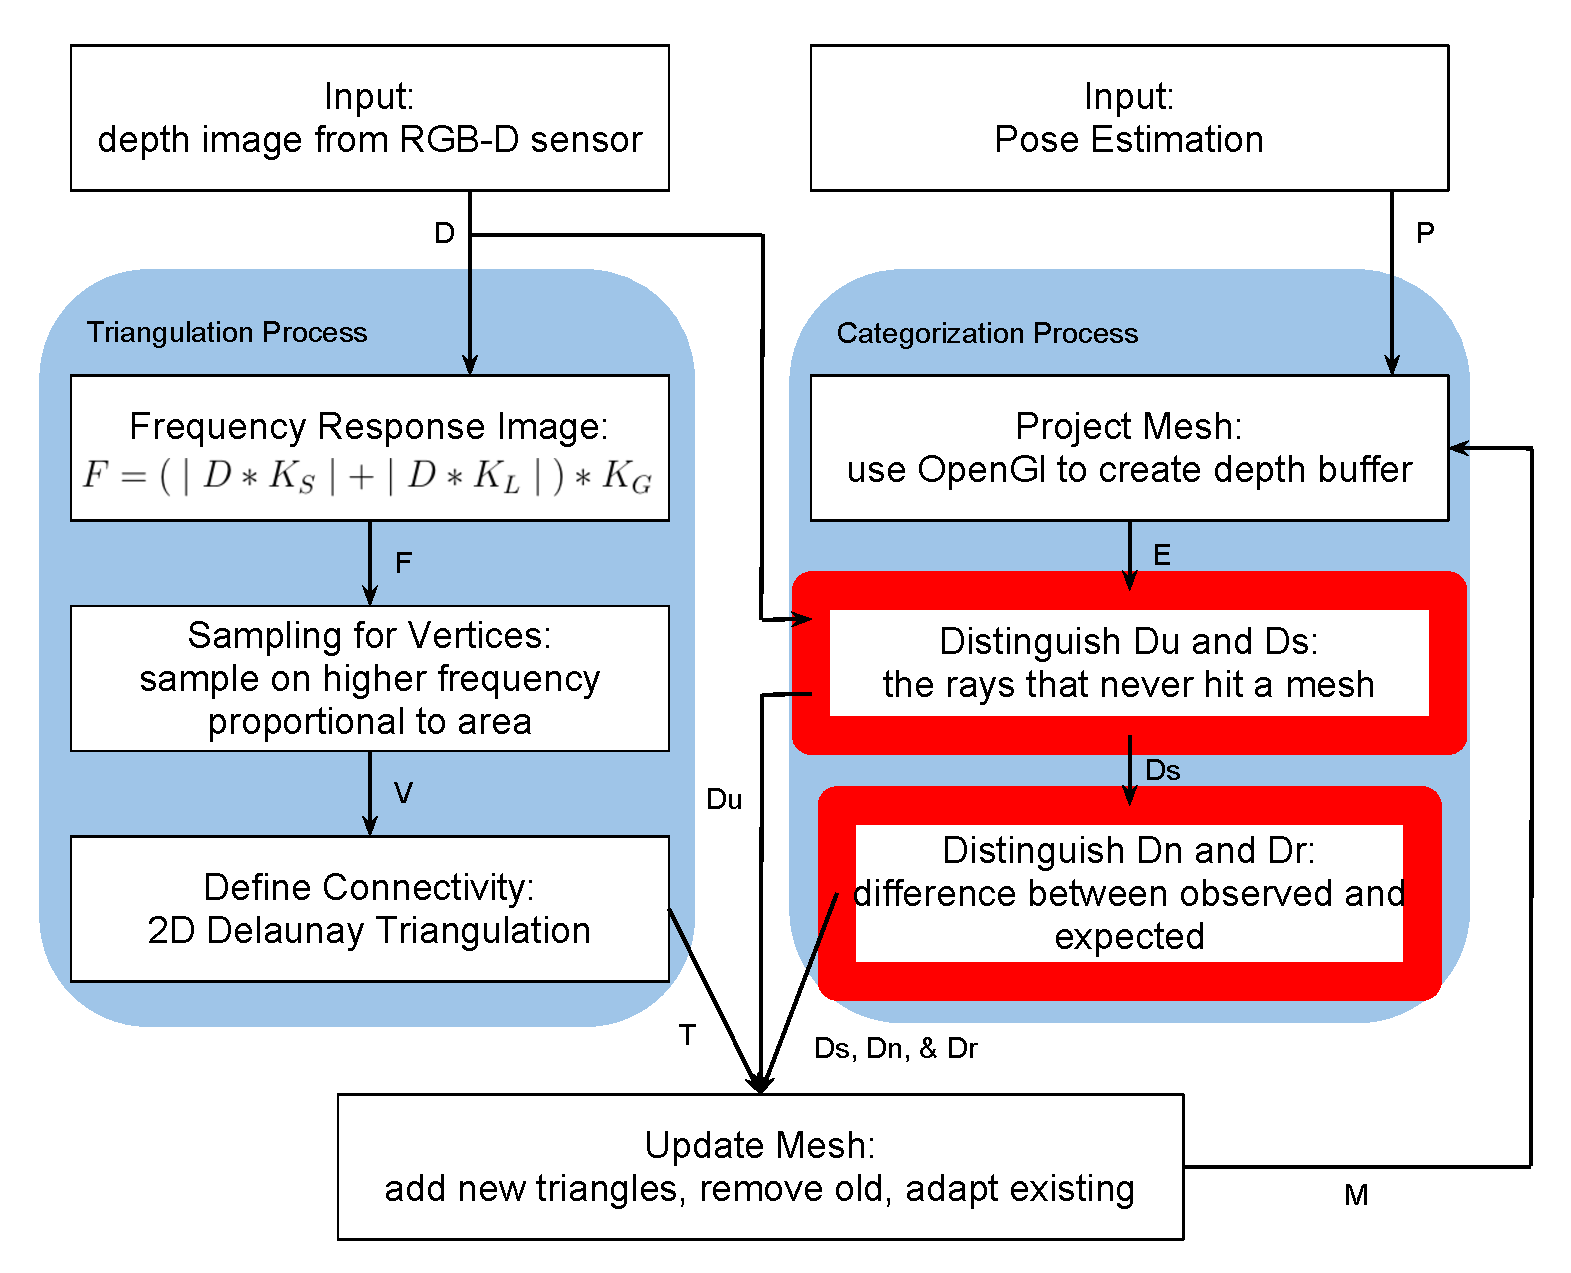
\includegraphics[width=\textwidth]{SDsort.pdf} 
  \end{center}
\column{.75\textwidth}
$D_u$ - region where rays never hit the mesh \\
$D_s$ - all valid measurements not containing $D_u$ \\
~\\
Define the change as $C = E - D_s$ \\
Perform blob analysis on $C$ (twice)  \\
~\\
$D_n$ - blobs with $C>\epsilon\ $; add triangles using $T$ \\
$D_r$ - blobs with $C<\epsilon\ $; remove triangles
\end{columns}
\end{frame}

\begin{frame}{Update mesh}
\vspace{-.2in}
\begin{columns}
\column{.25\textwidth}
  \begin{center}
  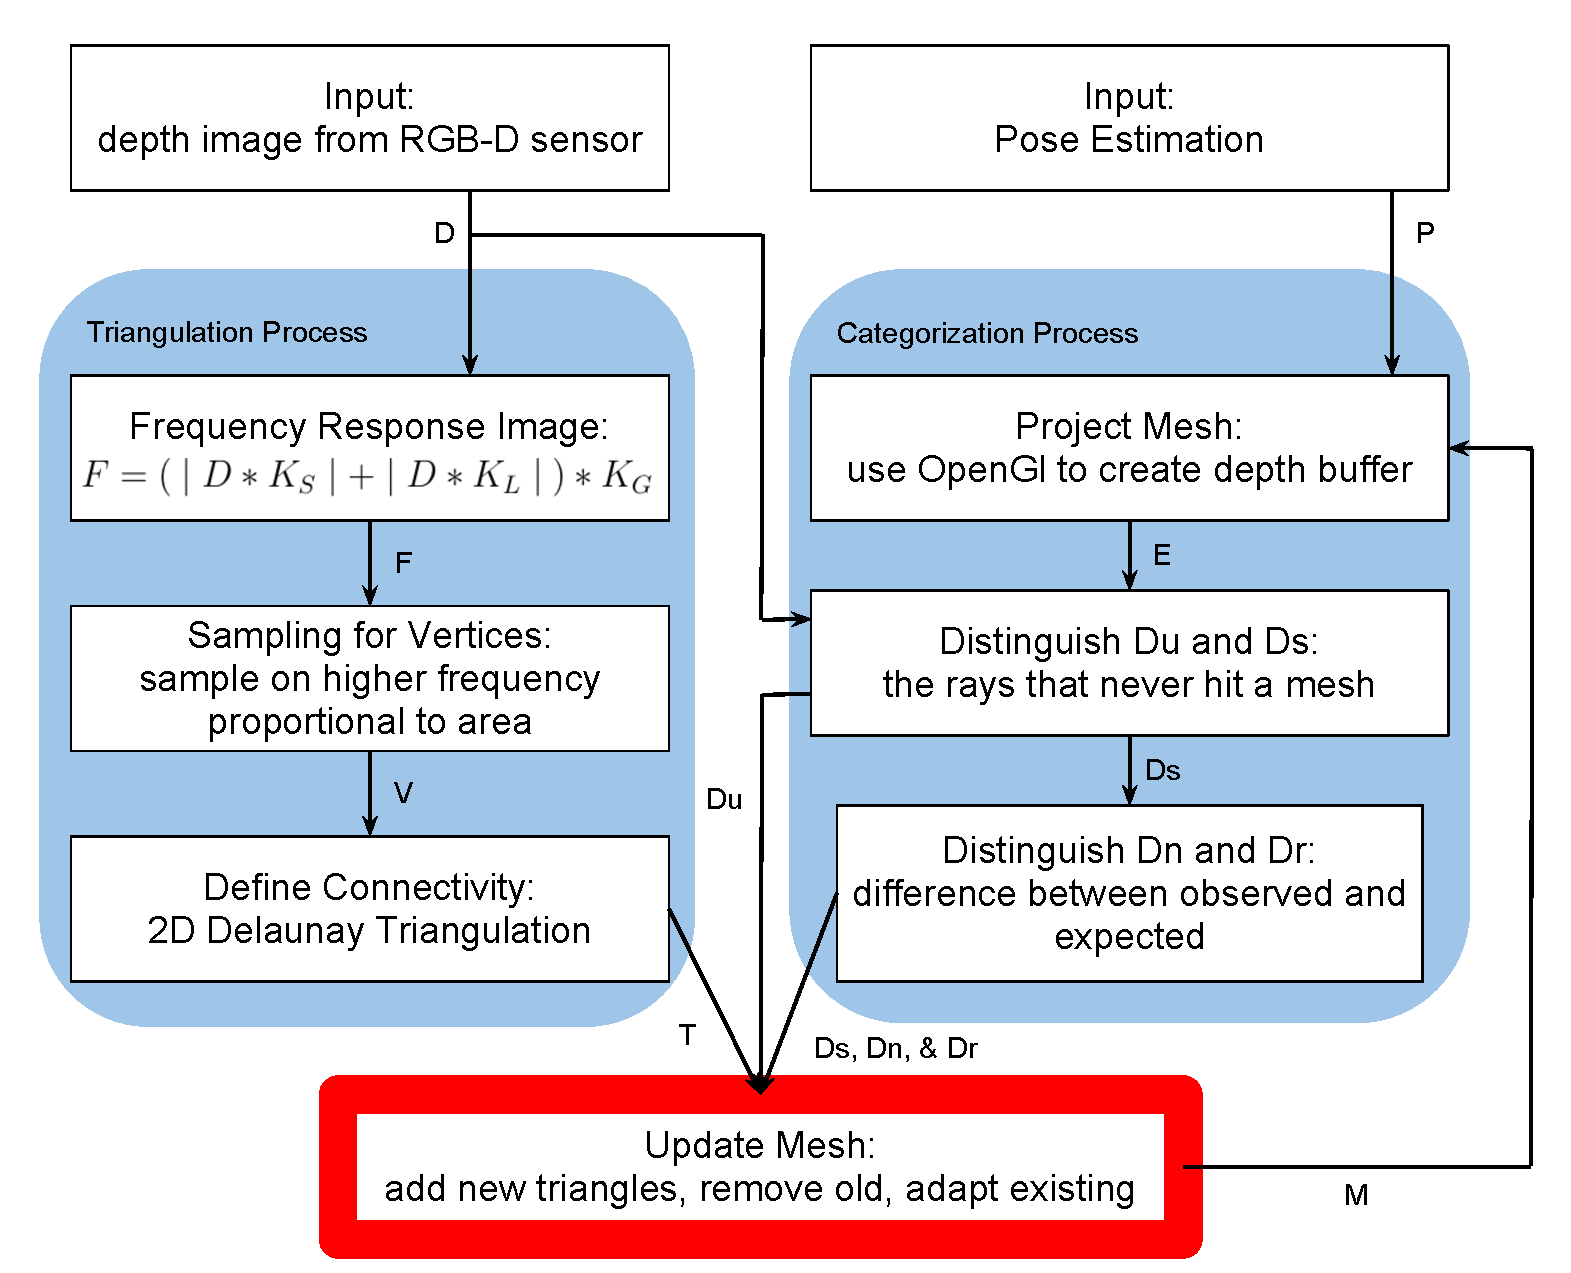
\includegraphics[width=\textwidth]{SDupdate.pdf} 
  \end{center}
\column{.75\textwidth}
$D_u$ - add triangles using $T$ \\
~\\
$D_s$ - adapt \\
~\\
$D_n$ - add triangles using $T$ \\
~\\
$D_r$ - remove triangles
\end{columns}
\end{frame}

\begin{frame}{Adapt position of each vertex with QEM}
\vspace{-.2in}
\begin{columns}
\column{.25\textwidth}
  \begin{center}
  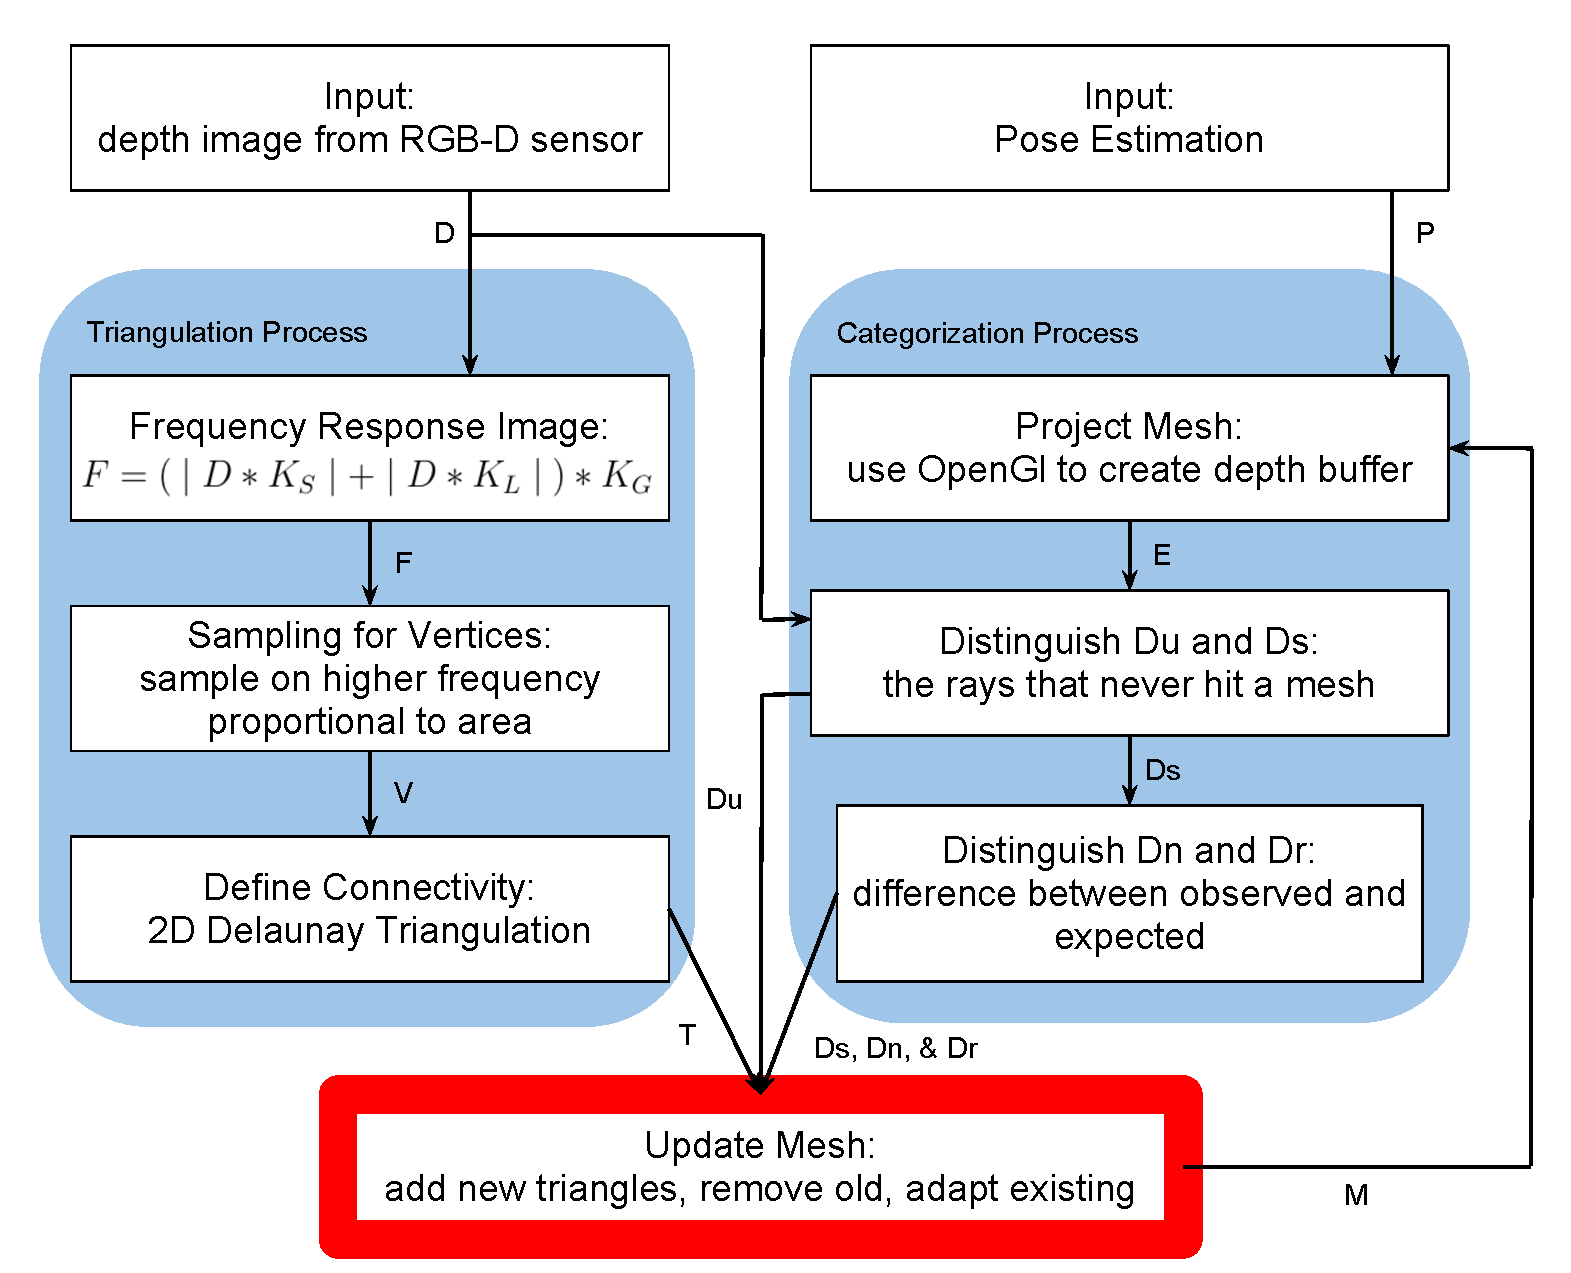
\includegraphics[width=\textwidth]{SDupdate.pdf} 
  \end{center}
\column{.75\textwidth}
  \begin{center}
  \begin{figure}
  \includegraphics<1>[width=\textwidth]{AM1.pdf} 
  \includegraphics<2>[width=\textwidth]{AM2.pdf} 
  \includegraphics<3>[width=\textwidth]{AM3.pdf} 
  \end{figure}
  \end{center}
\end{columns}
\end{frame}

\section{Testing}
\subsection{Simulation}

\begin{frame}{A simulation pipeline to test in}
\vspace{-.2in}
\begin{columns}
\column{.50\textwidth}
  \begin{center}
  \begin{figure}
  \includegraphics<1>[width=\textwidth]{Sim1.pdf} 
  \includegraphics<2>[width=\textwidth]{Sim2.pdf} 
  \includegraphics<3>[width=\textwidth]{Sim3.pdf} 
  \includegraphics<4>[width=\textwidth]{Sim4.pdf} 
  \includegraphics<5>[width=\textwidth]{Sim5.pdf} 
  \end{figure}
  \end{center}
\column{.50\textwidth}
Blender to define environment \\
~\\
OpenGl to generate z-buffer \\
~\\
Open in Matlab and add noise \\
~\\
Can project to get point cloud \\
~\\
Can apply a mesh
\end{columns}
\end{frame}

\subsection{Experiments}

\begin{frame}{What experiments will I do to validate my method?}
\begin{itemize}
\item Static scene; static object; static sensor \\
{\scriptsize Simple scene such as a cup on a table. Want to see convergence.} 
\item Static scene; static object; dynamic sensor \\
{\scriptsize Want to test ability to add triangles from unseen parts of environment.} 
\item Dynamic scene; static object; static sensor \\
{\scriptsize Detect new and removed objects from scene. Second cup and its removal.} 
\item Dynamic scene; dynamic object; static sensor \\
{\scriptsize A much more thorough test of removing and adding mesh.} 
\item Dynamic scene; dynamic object; dynamic sensor \\
{\scriptsize Complete system working in simulation.} 
\item Repeat with real data 
\end{itemize}
\end{frame}

\section*{Summary}

\begin{frame}{Summary}

  \begin{itemize}
  \item Importance of a mesh-based representation. 
  \item Main problem is measurement categorization.
  \item Can be solved with fast image based techniques.
  \end{itemize}
  
  % The following outlook is optional.
  \vskip0pt plus.5fill
  \begin{itemize}
  \item
    Things I'm scared of
    \begin{itemize}
    \item Merging boundaries of areas.
    \item Incremental adaptation with QEM.
    \item Pose estimation will never be that good.
    \end{itemize}
  \end{itemize}
\end{frame}

\begin{frame}
Questions or Comments?
  \begin{center}
  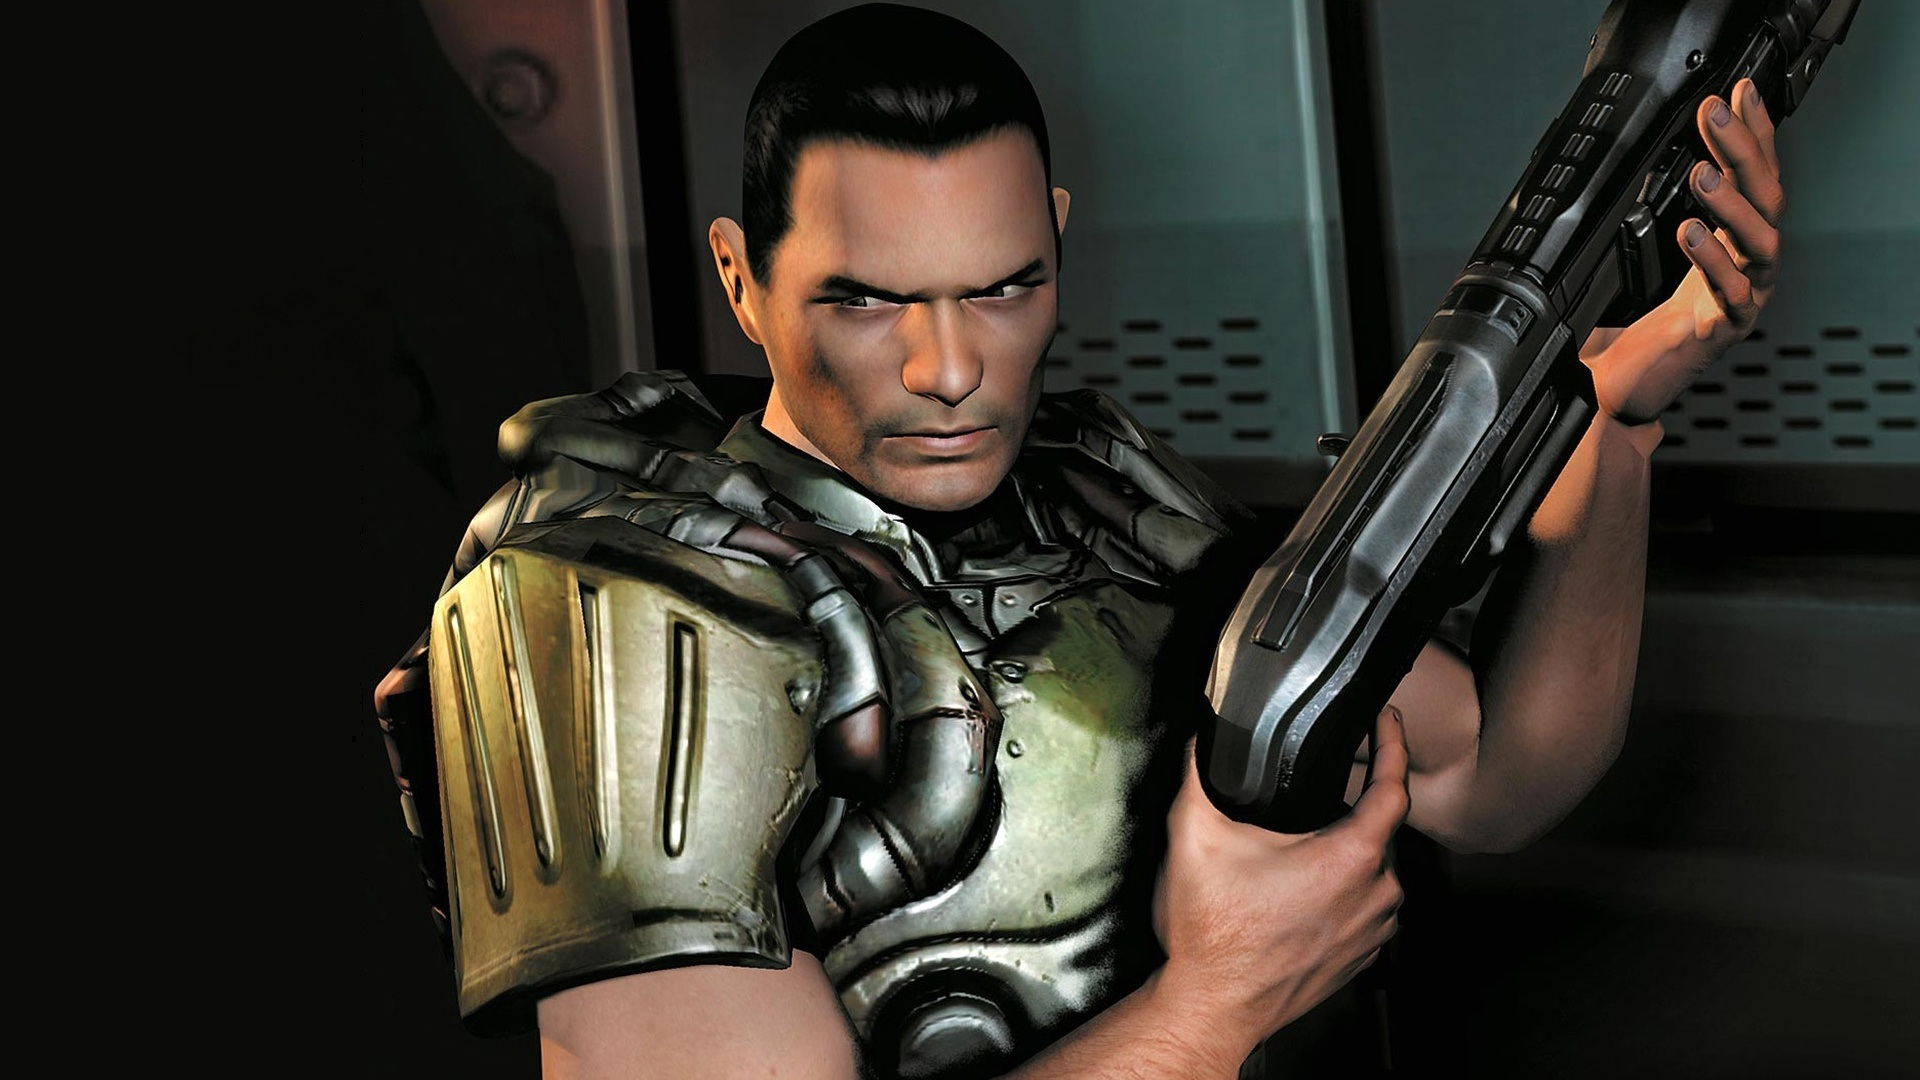
\includegraphics[width=\textwidth]{Doom3.jpg} 
  \end{center}
\end{frame}

\end{document}

%% All of the following is optional and typically not needed. 
%\appendix
%\section<presentation>*{\appendixname}
%\subsection<presentation>*{For Further Reading}
%
%\begin{frame}[allowframebreaks]
%  \frametitle<presentation>{For Further Reading}
%    
%  \begin{thebibliography}{10}
%    
%  \beamertemplatebookbibitems
%  % Start with overview books.
%
%  \bibitem{Author1990}
%    A.~Author.
%    \newblock {\em Handbook of Everything}.
%    \newblock Some Press, 1990.
% 
%    
%  \beamertemplatearticlebibitems
%  % Followed by interesting articles. Keep the list short. 
%
%  \bibitem{Someone2000}
%    S.~Someone.
%    \newblock On this and that.
%    \newblock {\em Journal of This and That}, 2(1):50--100,
%    2000.
%  \end{thebibliography}
%\end{frame}

%  You can create overlays\dots
%  \begin{itemize}
%  \item using the \texttt{pause} command:
%    \begin{itemize}
%    \item
%      First item.
%      \pause
%    \item    
%      Second item.
%    \end{itemize}
%  \item
%    using overlay specifications:
%    \begin{itemize}
%    \item<3->
%      First item.
%    \item<4->
%      Second item.
%    \end{itemize}
%  \item
%    using the general \texttt{uncover} command:
%    \begin{itemize}
%      \uncover<5->{\item
%        First item.}
%      \uncover<6->{\item
%        Second item.}
%    \end{itemize}
%  \end{itemize} 
